
%% General definitions
\documentclass{article} %% Determines the general format.
\usepackage{a4wide} %% paper size: A4.
\usepackage[utf8]{inputenc} %% This file is written in UTF-8.
%% Some editors on Windows cannot save files in UTF-8.
%% If there is a problem with special characters not showing up
%% correctly, try switching "utf8" to "latin1" (ISO 8859-1).
\usepackage[T1]{fontenc} %% Format of the resulting PDF file.
\usepackage{fancyhdr} %% Package to create a header on each page.
\usepackage{lastpage} %% Used for "Page X of Y" in the header.
%% For this to work, you have to call pdflatex twice.
\usepackage{enumerate} %% Used to change the style of enumerations (see below).

\usepackage{amssymb} %% Definitions for math symbols.
\usepackage{amsmath} %% Definitions for math symbols.

\usepackage{tikz}  %% Pagacke to create graphics (graphs, automata, etc.)
\usetikzlibrary{automata} %% Tikz library to draw automata
\usetikzlibrary{arrows}   %% Tikz library for nicer arrow heads
\usetikzlibrary{arrows.meta}   %% Tikz library for nicer arrow heads
\usetikzlibrary{positioning}   %% Tikz library for nicer arrow heads


%% Left side of header
\lhead{\course\\\semester\\Exercise \homeworkNumber}
%% Right side of header
\rhead{\authorname\\Page \thepage\ of \pageref{LastPage}}
%% Height of header
\usepackage[headheight=36pt]{geometry}
%% Page style that uses the header
\pagestyle{fancy}

\newcommand{\authorname}{Alex Lutsch\\Ephraim Siegfried }
\newcommand{\semester}{Fall Semester 2023}
\newcommand{\course}{Discrete Mathematics in Computer Science}
\newcommand{\homeworkNumber}{1}


\begin{document}



\section*{Exercise \homeworkNumber.1}

\begin{enumerate}[(a)]
	\item
	\item
\end{enumerate}



\section*{Exercise \homeworkNumber.2}

\begin{enumerate}[(a)]
	\item
	\item
\end{enumerate}



\section*{Exercise \homeworkNumber.3}

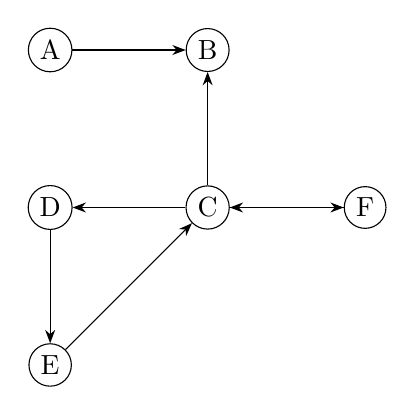
\begin{tikzpicture}[->,>=Stealth,node distance=2cm,on grid,auto]
	\node[circle, draw, inner sep=2pt] (A) {A};
	\node[circle, draw, inner sep=2pt] (B) [right=of A] {B};
	\node[circle, draw, inner sep=2pt] (C) [below=of B] {C};
	\node[circle, draw, inner sep=2pt] (D) [below=of A] {D};
	\node[circle, draw, inner sep=2pt] (E) [below=of D] {E};
	\node[circle, draw, inner sep=2pt] (F) [right=of C] {F};

	\draw (A) to (B);
	\draw (C) to (B);
	\draw (C) to (D);
	\draw (C) to (F);
	\draw (D) to (E);
	\draw (E) to (C);
	\draw (F) to (C);
\end{tikzpicture}


\section*{Exercise \homeworkNumber.4}



\section*{Exercise \homeworkNumber.5}

\begin{enumerate}[(a)]
	\item
	\item
	\item
	\item
\end{enumerate}



\end{document}
